Video notes (vid8.mp4)
\subsection*{Pole-Zero Analysis}

From our difference equation we have:

$Y(Z) = H(Z)X(Z)$

Which can derive the transfer function:

$H(Z) = \frac{B(Z)}{A(Z)}$

\textbf{ex: Our simplest lowpass}:

$y_n= x_n + x_{n - 1}$
$\leftrightarrow Y(Z) = X(Z) + Z^{-1}(Z)$
$H(Z) = 1 + Z^{-1}$


$H(Z) = \frac{B(Z)}{A(Z)}$

General causal LTI filter

\paulhint{frame 12a taken at 3:10}\\
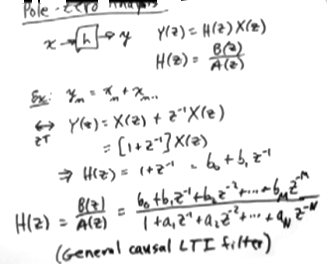
\includegraphics[scale=0.8]{frames/12a}

Without LTI, we don't have a transfer function. 

We pull out $b_0$ to make numerator monic, and write this:
% PB: How does this work? 
$b_0 \frac{(1 - b_1 Z^{-1})\cdots(1 - b_M Z^{-1})}
{(1 - p_1Z^{-1})\cdots{1 - p_N Z^{-1}}}$


Easier way to write it for pole zero analysis:

\paulhint{frame 12b taken at 5:43}\\
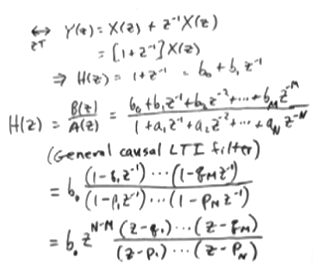
\includegraphics[scale=0.8]{frames/12b}

\subsection*{Freq Response}

The frequency response is the transfer function evaluated on the
unit circle: $H(z)\vert_{z = e^{j\omega T}}$

\paulhint{See eqn at 7:57, 12c}\\
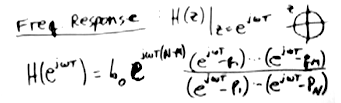
\includegraphics[scale=0.8]{frames/12c}

\subsection*{Graphical Amp Response}

%$G(\omega) = \vert H(e^{j\omegaT) \vert = \vert b_0\vert \cdots $


\paulhint{frame 12d taken at 5:43. use eqn written}\\
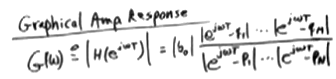
\includegraphics[scale=0.8]{frames/12d}

By graphical, we mean you can now into the complex plane and draw
the unit circle and pick a point on the unit circle. 

To look at our frequency response, we let omega grow from zero to 
half the sampling rate. We can now see what the magnitude frequency response
is as a function of the poles and zeros just looked at as distances. 

$q1$ is numerator

The poles are conjugate pairs (that's what he drew them as). 

The evaluation can done graphically: what is the vector $e^{j\omega T} - q_1$?

It is the arrow from $q_1$ to that point (he draws an arrow). That is the
difference vector. if $q_1$ is added to this difference vector, you get 
$e^{j \omega T}$. 

Normally this method is used for visualizing it graphically in your head. At DC
you are closes to the zero and far from the poles. As you go up, things kind of 
stay the same. when you whip around to the pole, you are going to be 
dividing by a very short distance to that pole, so you can see the resonance that way.
\\
When you fly by a pole, you get a big resonance, or gain peak. 
\\
\paulhint{frame 12e taken at 13:22. mainly for chart}\\
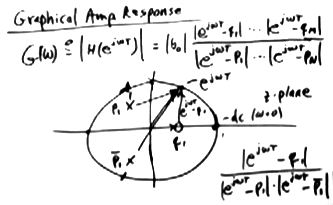
\includegraphics[scale=0.8]{frames/12e}
\\
Traditionally, a zero is denoted with an open zero, and a pole is denoted with an X. 
\\
Typically, we normally go through half the circle because the filter is real
and the negative response is the complex conjugate of the postive frequency 
response.\\

\paulhint{REWATCH: 15:02 is a little unclear (book example). rewatch this and see
if it visually "clicks"} 

\subsection*{Graphical Phase Response}
Same story, but angle instead of magnitude. 

$\theta(\omega) = \angle H(e^{j\omega T})$ \\

We need...\\
Angle $b_0$ will be $0$ or $\pi$ if it is real. \\
Angle for the unit modular constant/term $e^{j\omega T (N - M)}$\\

With amp response, we were multiplying by the zero distances and dividing
by the pole distances, now we want to sum the angles for the zeros, and subtract
for the poles. 


\paulhint{frame 12f taken at 13:22. note the chart.. it is also in the book 
(figure 8.4)}\\
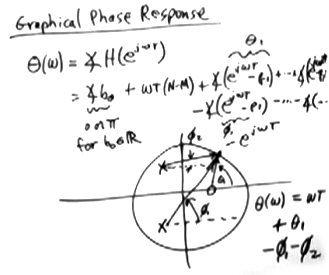
\includegraphics[scale=0.8]{frames/12f}

To reiterate, this approach is really only to visualize what is going on in 
our heads. Computers are more practical.  

In figure 8.5, the phase response has a distorted sinusoidal shape with
the particular point. Qualitatively, our point is the maximum. Why is it the 
maximum? In 8.4, The DC, theta 1 is zero and theta 2 are zero. theta 3, 4 cancel. You
get a zero dc phase. You also get a zero phase at half the sampling rate. 

\paulhint{REWATCH: at around 12:00 he starts explaining how to visually see the
phase, rewatch this as it's a good visualization. You'll want to develop 
this kind of insight.}

